\documentclass[10pt,a4paper]{report}
\usepackage[latin1]{inputenc}
%\usepackage[utf8x]{inputenc}
\usepackage[english]{babel}
\usepackage{amsmath}
\usepackage{amsfonts}
\usepackage{amssymb}
\usepackage{graphicx}
\usepackage{verbatim}
\usepackage[left=1.5cm,right=1.5cm,top=2.5cm,bottom=2.5cm]{geometry}

\usepackage{float}
\usepackage{multirow}
\usepackage{graphicx}
\usepackage{subcaption}

\pagenumbering{gobble}

\DeclareMathOperator{\ind}{\perp \!\!\! \perp}



% Le document est sur 6 pages organisées comme ci-dessous :
% 1 3 5
% 2 4 6
\begin{document}

\begin{center}
\resizebox{\linewidth}{!}{\itshape \textbf{Generalization and}}
\end{center}
\vspace{80pt}

\begin{center}
\Huge{\textit{Introduction}}
\end{center}
\vspace{20pt}

\Large{
	
	Hidden Markov Models (HMMs) are widely used for probabilistic models of time series data. Here we used a generalization of HMMs called factorial hidden Markov model, in which a state $S_t$ corresponding to an hidden variable is now represented by a collection of states $S_t = \left(S_t^{(1)},\dots,S_t^{(M)}\right)$ each of which can take $K^{(m)}$ values (figure (a)). Here we consider the case where $K = K^{(m)}$ for all $m$. Furthermore, we assume that $\{(S_t^{(m)})_{t=0}^T\}_{m=0}^M$ are independent Markov chains and that the observation $y_t$ are Gaussian random vector whose mean is a linear function of the hidden variables and have the same covariance matrix $C$.
	\newline
	\newline
	
	}

\begin{figure}[h]
	\centering
	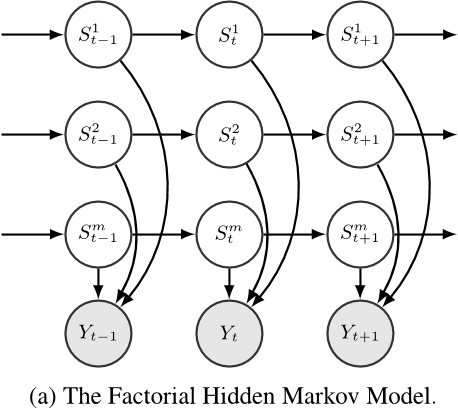
\includegraphics[width=0.6\textwidth]{fHMM.png}
	%\centerline{Factorial Hidden Markov Model}
	\label{fig:a}
\end{figure}


\newpage
\begin{center}
\Huge{\textit{Inference and learning}}
\end{center}
\vspace{20pt}

\Large{

Here we want to learn the parameters of a factorial HMM for a given structure. For that we use the EM algorithm to estimate them. While the M step is simple and tractable, the E step is computationally more difficult. We have four options:

\begin{itemize}
	\item[-]Exact inference: it is computationally intractable for a big model.
	\item[-]Inference using Gibbs sampling.
	\item[-]Completely factorized variational inference: we approximate the posterior distribution by a tractable distribution and we make the assumption that all the hidden variables are independent.
	\item[-]Structured variational inference: same as above but we take into account the structure of the hidden variables (figure(b)).
\end{itemize}
\vspace{20pt}
}

\begin{figure}[h]
	\centering
	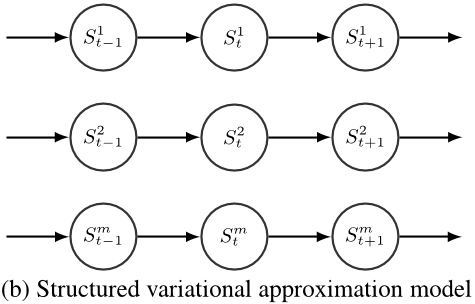
\includegraphics[width=0.7\textwidth]{sva.png}
	%\centerline{Factorial Hidden Markov Model}
	\label{fig:b}
\end{figure}








\newpage
\begin{center}
\resizebox{\linewidth}{!}{\itshape \textbf{acceleration of HMMs}}
\end{center}
\vspace{5pt}
\begin{center}
	\LARGE{Matthieu Jedor \& Alban Pierre}
	\vspace{15pt}
	
	\Large{Keywords: Hidden Markov models, time series, EM algorithm, graphical models, Bayesian networks, mean field
theory}
\end{center}
\vspace{30pt}
\begin{center}
\Huge{\textit{Experiments on synthetic data}}
\end{center}
\vspace{20pt}
%\Large{
	
%	We generate synthetic datasets using a factorial hidden Markov model and then we tried to learn the parameters with our 4 algorithms. Figure (c) shows the log-likelihood accross iterations and figure (d) shows the results in terms of centers found.
	
%}

% TODO add log-likelihood plots and time of computation, and the protocol of experimentations

Here, we generate synthetic datasets using a factorial hidden Markov model and then we tried to learn the parameters with our 4 algorithms. The data were generated from a factorial HMM structure with M Markov chains and each of the state variables could take K discrete values. We choose $C$ to be a multiple of the identity matrix $C = 0.01 I$. W was sampled from a standard normal distribution and the other parameters from a uniform $[0,1]$ distribution and the transition matrix and priors were then normalized to satisfy the sum-to-one constraints. The training and test sets consisted of 200 Gaussian vector with dimension 2. 

Table 1 shows the results averaged over 15 runs for each algorithms on each of the four problem sizes. 

\begin{table}[h]
\centering
\begin{tabular}{cclll}
\hline
\ttfamily M & \ttfamily K & \ttfamily Algorithm & \ttfamily Training Set & \ttfamily Test Set \\
\hline
\multirow{4}{*}{3}  & \multirow{4}{*}{2} 
& \multicolumn{1}{c}{Exact} & \multicolumn{1}{c}{0.84}  & \multicolumn{1}{c}{0.95}
\\ \cline{3-5}
&	 & \multicolumn{1}{c}{Gibbs} & \multicolumn{1}{c}{1.74} & \multicolumn{1}{c}{1.87}
\\ \cline{3-5}
&   & \multicolumn{1}{c}{CFVA} & \multicolumn{1}{c}{1.09} & \multicolumn{1}{c}{1.24} 
\\ \cline{3-5}
&    & \multicolumn{1}{c}{SVA} & \multicolumn{1}{c}{1.46} & \multicolumn{1}{c}{1.61} \\ 
\hline
  \multirow{4}{*}{3}  & \multirow{4}{*}{3} 
& \multicolumn{1}{c}{Exact} & \multicolumn{1}{c}{0.96}  & \multicolumn{1}{c}{1.20}
\\ \cline{3-5}
&	 & \multicolumn{1}{c}{Gibbs} & \multicolumn{1}{c}{2.40} & \multicolumn{1}{c}{2.72}
\\ \cline{3-5}
&   & \multicolumn{1}{c}{CFVA} & \multicolumn{1}{c}{1.09} & \multicolumn{1}{c}{1.23} 
\\ \cline{3-5}
&    & \multicolumn{1}{c}{SVA} & \multicolumn{1}{c}{1.43} & \multicolumn{1}{c}{1.51} \\ 
\hline
\multirow{4}{*}{5}  & \multirow{4}{*}{2} 
& \multicolumn{1}{c}{Exact} & \multicolumn{1}{c}{2.17}  & \multicolumn{1}{c}{2.41}
\\ \cline{3-5}
&	 & \multicolumn{1}{c}{Gibbs} & \multicolumn{1}{c}{3.55} & \multicolumn{1}{c}{3.88}
\\ \cline{3-5}
&   & \multicolumn{1}{c}{CFVA} & \multicolumn{1}{c}{1.37} & \multicolumn{1}{c}{1.64} 
\\ \cline{3-5}
&    & \multicolumn{1}{c}{SVA} & \multicolumn{1}{c}{1.44} & \multicolumn{1}{c}{1.61} \\ 
\hline
\multirow{4}{*}{5}  & \multirow{4}{*}{3} 
& \multicolumn{1}{c}{Exact} & \multicolumn{1}{c}{4.10}  & \multicolumn{1}{c}{4.45}
\\ \cline{3-5}
&	 & \multicolumn{1}{c}{Gibbs} & \multicolumn{1}{c}{3.82} & \multicolumn{1}{c}{4.12}
\\ \cline{3-5}
&   & \multicolumn{1}{c}{CFVA} & \multicolumn{1}{c}{3.97} & \multicolumn{1}{c}{4.38} 
\\ \cline{3-5}
&    & \multicolumn{1}{c}{SVA} & \multicolumn{1}{c}{4.01} & \multicolumn{1}{c}{4.31} \\  
\hline 
\end{tabular}
\caption{Comparison of the factorial HMM on four problems of varying size. The log-likelihood is measured in bits per observation relative to the log-likelihood under the true generative model.}
\label{tab:xxx}
\end{table}

\newpage

\begin{figure}[ht] 
  \begin{subfigure}[b]{0.5\linewidth}
    \centering
    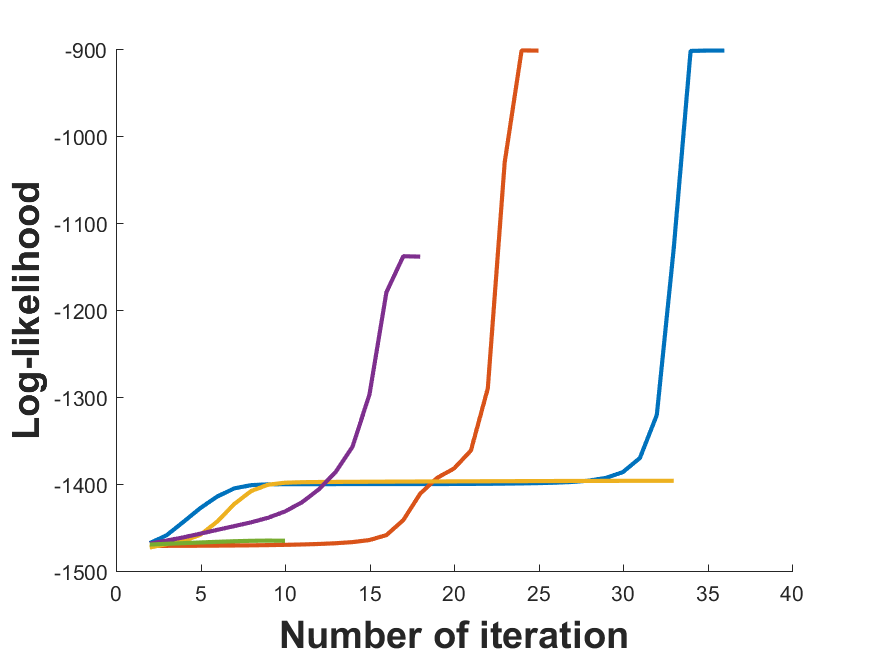
\includegraphics[width=0.75\linewidth]{init_fhmm.png} 
    \caption{Exact} 
    \label{fig7:a} 
    \vspace{4ex}
  \end{subfigure}%% 
  \begin{subfigure}[b]{0.5\linewidth}
    \centering
    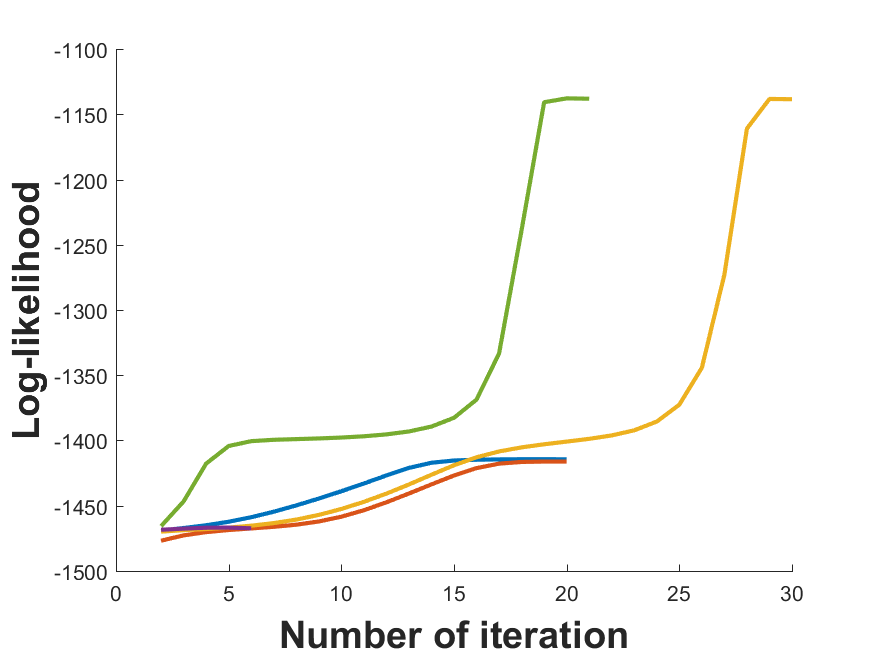
\includegraphics[width=0.75\linewidth]{init_gibbs.png} 
    \caption{Gibbs} 
    \label{fig7:b} 
    \vspace{4ex}
  \end{subfigure} 
  \begin{subfigure}[b]{0.5\linewidth}
    \centering
    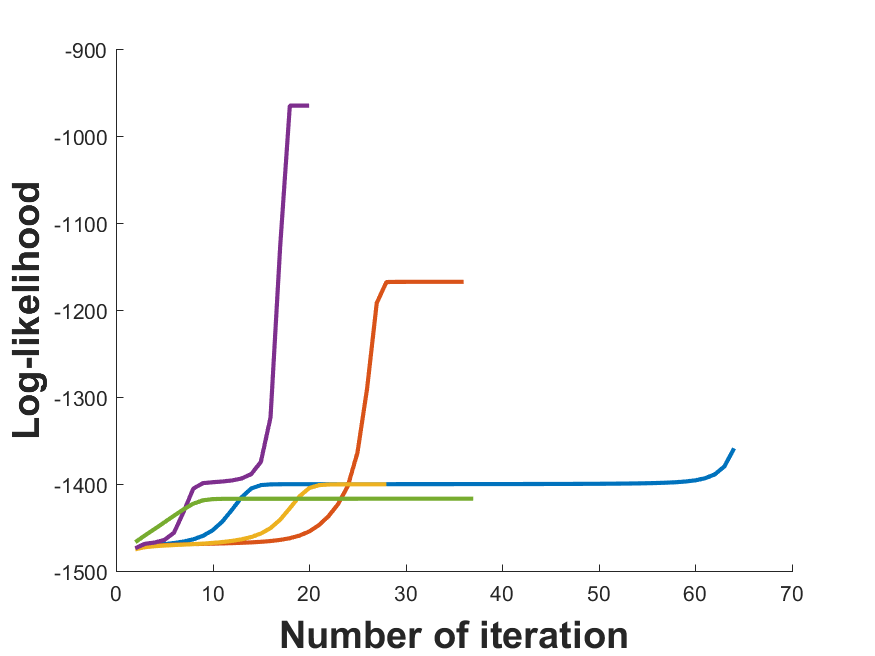
\includegraphics[width=0.75\linewidth]{init_cfva.png} 
    \caption{CFVA} 
    \label{fig7:c} 
  \end{subfigure}%%
  \begin{subfigure}[b]{0.5\linewidth}
    \centering
    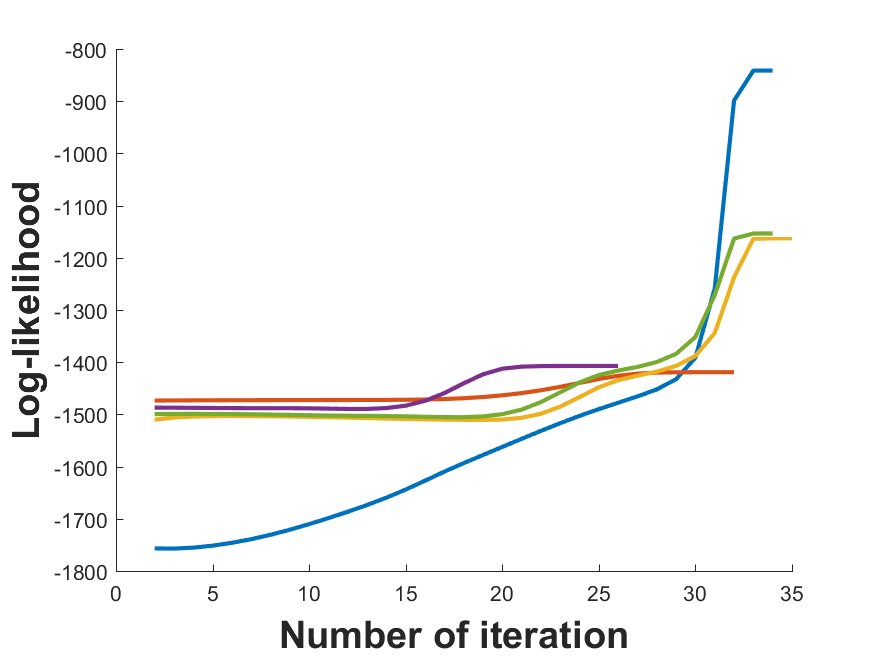
\includegraphics[width=0.75\linewidth]{init_sva.png} 
    \caption{SVA} 
    \label{fig7:d} 
  \end{subfigure} 
  \caption{Learning curves for five runs of each of each of the four learning algorithms}
  \label{fig7} 
\end{figure}


\begin{figure}[H]
	\centering
	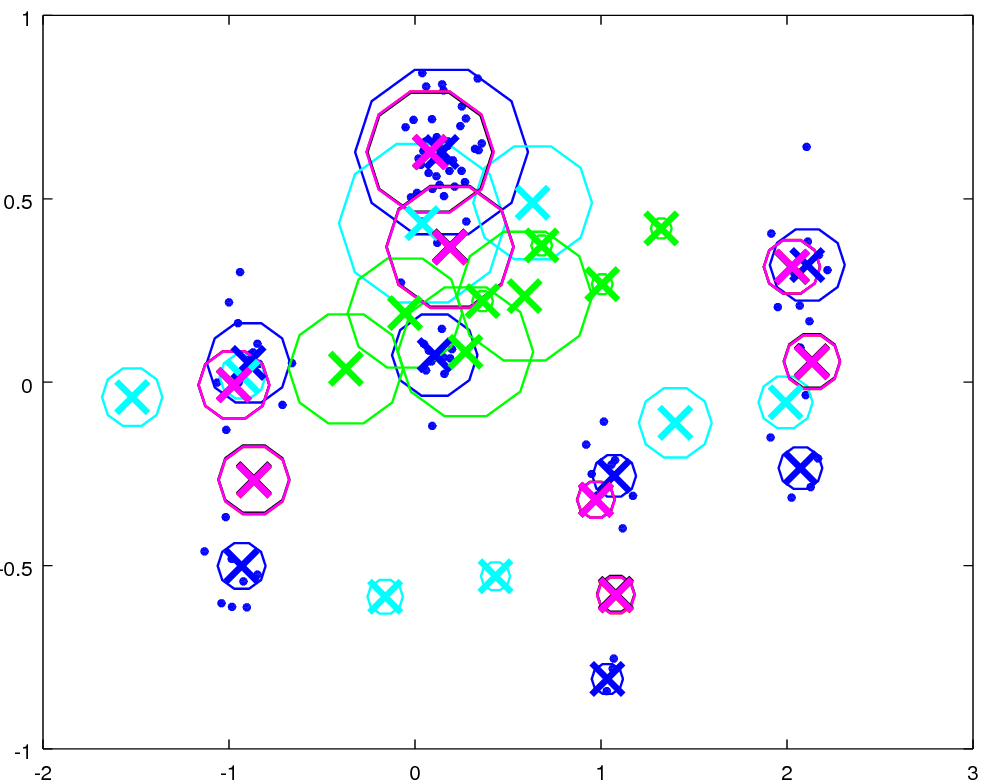
\includegraphics[width=0.8\textwidth]{fig11.png}
	\centerline{\Large{(d) Centers for synthetic data}}
	\label{fig:c}
\end{figure}
\begin{center}
	Cross = centers, Circles = probabilities of each center
	
	Blue = True parameters
	
	Light Blue = Kmeans Initialization
	
	Violet = FHMM, CFVA, SVA (they found the same result)
	
	Green = Gibbs sampling
	
\end{center}
\vspace{30pt}

The initialization of parameters is crucial. With a random initialization, we achieved poor results as half centers found by our algorithms or less matched the whole data and the other half ended in the middle of nowhere. So we used a recursive K-means initialization, which works as follow : (with $W$ defining the centers : $\mu_t = W*S_t$ ; and $P$ the transition matrix)

\begin{verbatim}
For m = 1 to M
     k = kmeans with K centers
     Superpose each cluster found
     The m-th set of K columns of W = k
     The m-th set of K lines of P = probabilities of clusters k
endFor
\end{verbatim}






\clearpage
\begin{center}
\resizebox{\linewidth}{!}{\itshape \textbf{using factorial HMMs}}
\end{center}
\vspace{80pt}
\begin{center}
\Huge{\textit{Experiments on real data}}
\end{center}
\vspace{20pt}

We applied the structural variational approximation on real data. First we choose the dataset "Activity Recognition from Single Chest-Mounted Accelerometer Data Set" from UCI Repository, which records the acceleration of persons during different activities such as walking, going up/down stairs or working at computer. We tried to learn parameters of each of theses activities, and then for a new activity we compute the log-likelihood of each set of parameters, and the set of parameters that gave the biggest log-likelihood would be the recognized activity. In practice the data is not separated in several gaussians (figure (e)) so it performs poorly at recognizing activities.

\begin{figure}[h]
	\centering
	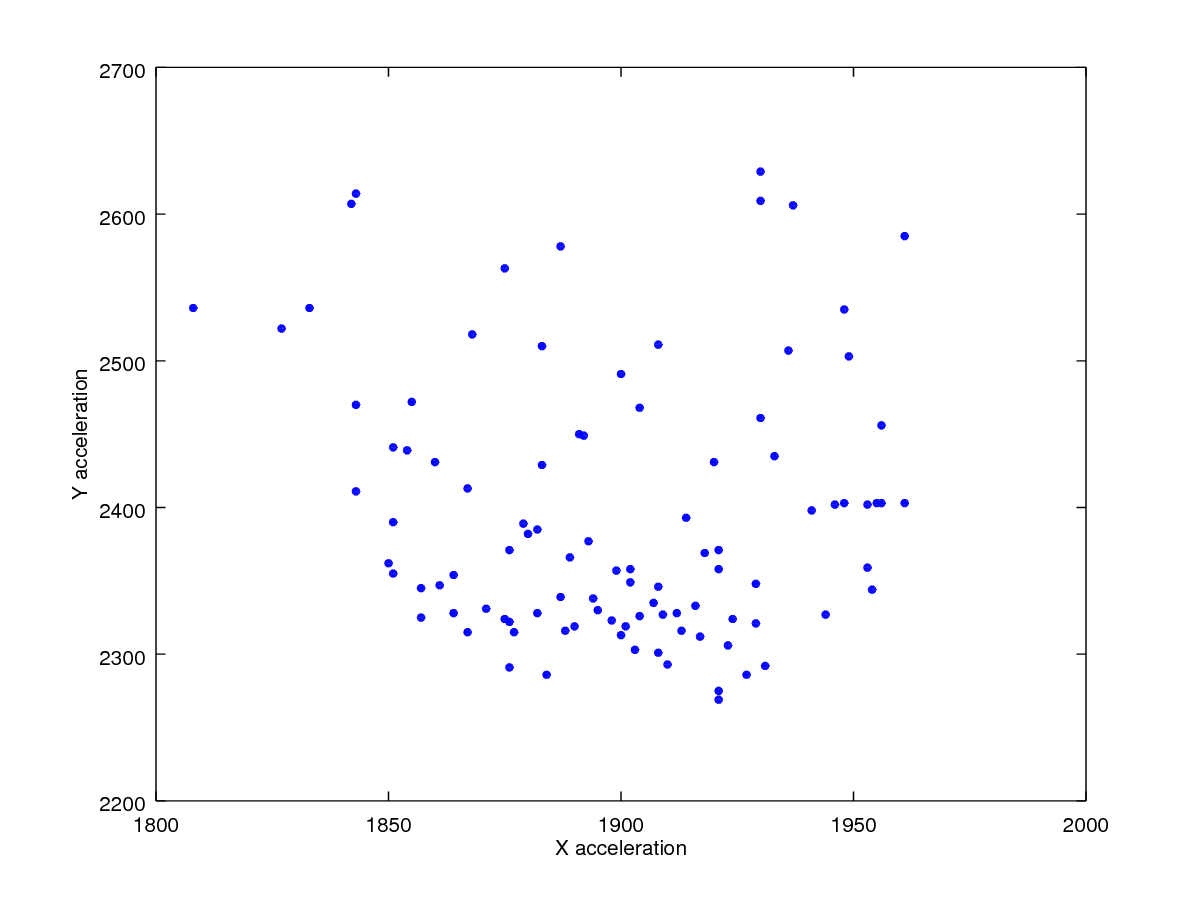
\includegraphics[width=0.7\textwidth]{standing.png}
	\centerline{\Large{Example of data from Single Chest-Mounted Accelerometer Data Set}}
	\label{fig:e}
\end{figure}

\newpage
Then we tried another dataset : CalIt2 Building People Counts Data Set, which counts the number of persons that come in and out of a building. So we expect different cluster such as the beginning of the day when every one comes in and nobody comes out, the night when there is no mouvement, or the lunch pause when there is many people coming both ways. Unfortunately, here again the dataset does not seem very structured (figure (f)).

\begin{figure}[h]
	\begin{minipage}[b]{.48\linewidth}
		\vspace{10pt}
		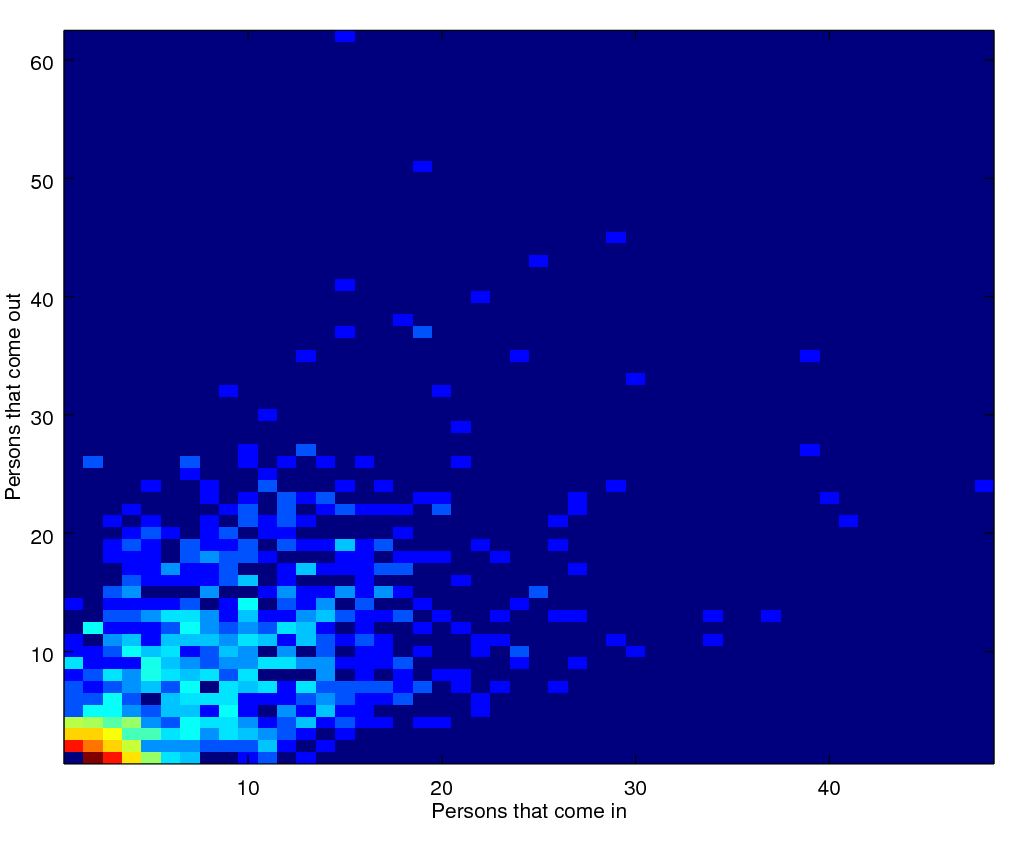
\includegraphics[width=1.0\textwidth]{building.png}
		%  \vspace{1.5cm}
		\begin{center}
			\large{(f) Example of data from CalIt2 
			Building People Counts Data Set}
		\end{center}\medskip
	\end{minipage}
	\hfill
	\begin{minipage}[b]{0.48\linewidth}
		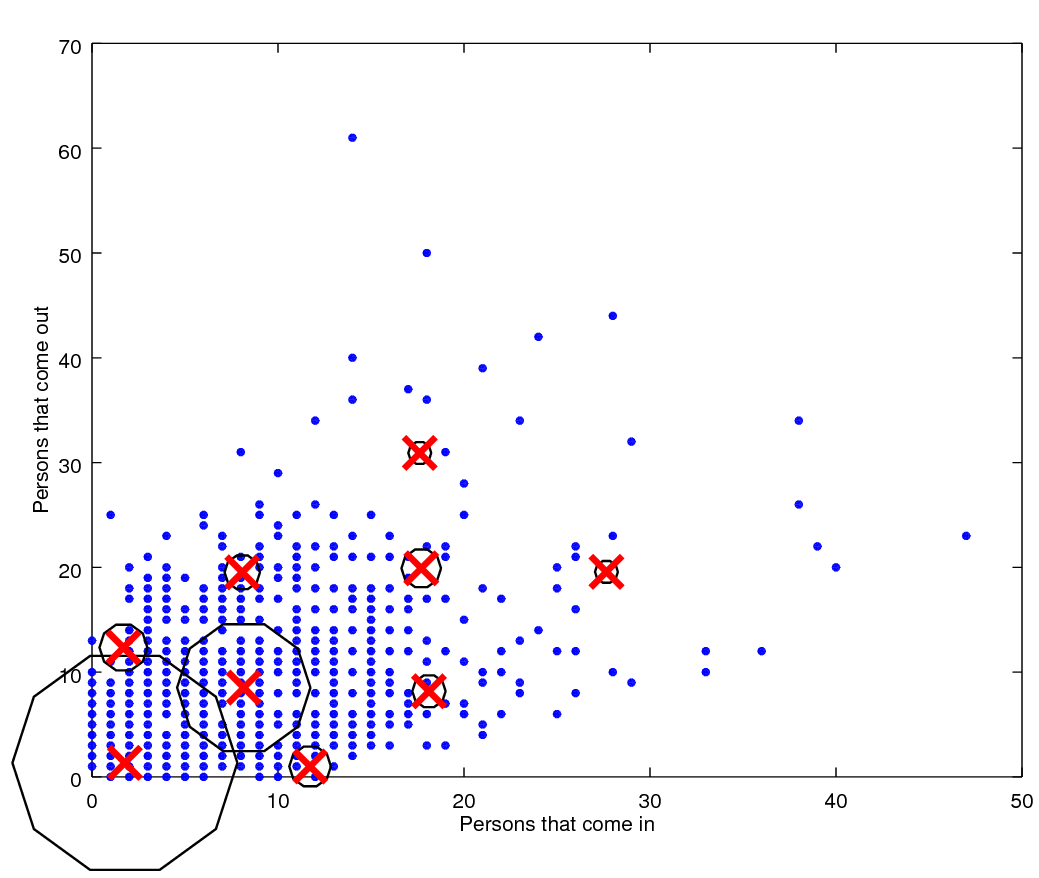
\includegraphics[width=1.0\textwidth]{expe4.png}
		%  \vspace{1.5cm}
		\begin{center}
			\large{(g) Centers found by structural
				variational approximation}
			\end{center}\medskip
	\end{minipage}
	\label{fig:f}
\end{figure}

\vspace{30pt}
\begin{center}
	\Huge{\textit{Conclusion}}
\end{center}
\vspace{20pt}

HMMs are used a lot and the factorial HMMs offers a generalization and a speed up in learning time-series probabilistics models. But in order to be efficient, the data must have regular cluters, organized in some patterns and few dataset have theses patterns. Moreover, the assumption that the covariance matrix is the same for each cluster seems false.
\newline

Thus, further work should relax the covariance matrix equality for each cluster. It may also be helpful to add some links between each parallel HMM to match more complicated data, without being limited to match patterns.

\iffalse

\begin{figure}[h]
	\centering
	\includegraphics[width=1.0\textwidth]{P2.png}
	\centerline{Paramètres utilisés pour calculer les probabilités des états cachés}
	\label{fig:d}
\end{figure}


\begin{tabular}{lcc}
	& Entrainement & Test \\
	EM mixture de gaussiennes & -2371 & -2453 \\
	EM chaine de Markov cachée & -1899 & -1957 \\
\end{tabular}
\newline

\fi

\end{document}
